\documentclass[14pt,a4paper]{article}
\usepackage{txfonts}
\usepackage{url}
\usepackage[colorlinks, citecolor=blue, urlcolor=blue]{hyperref}
\usepackage[utf8]{inputenc}
\usepackage[spanish]{babel}
\usepackage{amsmath}
\usepackage{amsfonts}
\usepackage{amssymb}
\usepackage{makeidx}
\usepackage{graphicx}
\usepackage{lmodern}
\usepackage{kpfonts}
\usepackage{fourier}
\usepackage[left=2cm,right=2cm,top=2cm,bottom=2cm]{geometry}
\author{Rodriguez Lopez Francisco Javier}


\begin{document}
\begin{center}
\paragraph{\large UNIVERSIDAD POLITECNICA DE LA ZONA METROPOLITANA DE GUADALAJARA}


\includegraphics[scale=1]{Upzmg.png} 
\end{center}
\begin{center}
\textbf{\LARGE Avance 1}\\
\end{center}
\begin{center}
\textbf{\LARGE Brazo Robotico}
\end{center}


\large{Integrantes:}\\
\large{Guzman Vazquez Jaime Alan.\\
Perez de Alba Santiago Eduardo.\\
Romero Jauregui Osvaldo.\\
Cabrera Gutierrez Raul.\\
Gutierrez Olivares Rogelio.\\
Rodriguez Lopez Francisco Javier.\\

Fecha: 20 de septiembre del 2019.\\

Curso: Sep-Dic 2019.\\

Carrera: Ingenieria en Mecaronica.\\

Docente: Moran Garabito Carlos Enrique.\\
Vazquez Alcaraz Laura Eugenia.}

\newpage

\section{Titulo de Proyecto:}

Brazo robotico multidiplicinario con acoplamiento para diferentes tareas de grado industrial con gran libertad de movimiento y solucion de problemas industriales.


\section{Planteamiento del problema:}

\subsection{Reunir.}
Para poner cierto contexto el proyecto se presentaran las diferentes cuestiones que orientan a realizar esta proyecto  por diferentes cuestiones los brazos roboticos son utiles y en el ambito empresarial estos son muy utilizados por su versatilidad y facil programacion.

\subsection{Determinar.}
El brazo robotico tiene gran importancia en la industria en general por esto se alento a realizar esto debido a que tienen gran potencial y podria ser utilizado en diferentes ambitos debido a su disposicion y versatilidad.

\subsection{Identificar}
las dificultades de este proyecto a futuro podria ser cuestiones como el presupuesto podria ser una de las mayor dificultades, a esto se le podria sumar cuestiones como la cotizacion de todos los materiales y precios para conseguir las mejores ofertas asi como los componentes\\
otra de las dificultades podria ser la compatibilidad con las diferentes accesorios para las que podria ser utilizado este brazo debido a que los tipos de piezas empleadas para las diferentes cuestiones de la industria. 

\subsection{Proponer}
Estas dificultades son de gran importancia para este proyecto debido a que en cuestion de presupuesto o de inversion para el proyecto debido a que se necesitan piezas relativamente costosas debido a que se necesitan componentes de calidad para garantizar la cuestion de la durabilidad.

\subsection{Encontrar}
para las dificultades anteriores propone las distintas soluciones para la cuestion de el presupuesto la solucion a esto seria abaratar costos creando por ejemplo la base de el brazo de materiales reciclados o cuestiones similares ademas de tener una planificacion en cuestion del presupuesto con un ingreso a plazos, como el proyecto esta basado a un año la administracion de este proyecto, esto podria solventar el problema de el presupuesto.\\
\\Para resolver el problema de la compatibilidad con las piezas de otros fabricantes, se implementara un sistema de intercambio de cabezales para lograr que el brazo robotico pueda ser compatible con estas diferentes piezas ademas de generar acoplamientos o adaptadores para el brazo robotico. 

\subsection{Hallar}
Las diferencias que se encuentran en el campo industrial podriamos hallar 
que el proyecto es completamente echo con componentes comerciales mientras que los brazos roboticos industriales estan generados a mucho mayor costo ademas de componentes de grado industrial y de mayor durabilidad y calidad, sin embargo este proyecto puede ser tomado a manera de prototipo podria ser llevado a gran escala.  

\subsection{Analizar} 
El sustento en el que se basan los datos anteriores seria basado en el mercado actual asi como los datos obtenidos del mercado al igual que el funcionamiento de estos y los componentes en estimados asi como su precio en diferentes tiendas, asi como en linea.\\
los puntos anteriores esta basados en conocimientos adquiridos mediante el estudio de la implementacion de estos en los medios industriales, al igual que el funcionamiento de estos fueron previamente estudiados.

\section{Formulacion de Problema:}

En este apartado, se estarn viendo las preguntas que se puedan generar respecto a un futuro, dentro del proyecto:\\


¿Es el brazo robotico la herramienta mas eficaz para sustituir al ser humano en la industria?\\
¿Es buena idea suplementar este tipo de dispositivos para otras actividades ademas de industriales?\\
¿El brazo es algo eficiente a la hora de realizar su tarea?\\
¿Se puede, implemetar para tareas complejas que sean de eficiencia y rapidez?\\
¿Es buena idea de la implementacion de automatizacion con este tipo de dispositivos? 

\section{Objetivo General:}

Creacion de un brazo robòtico con la finalidad de adaptacion a tareas complejas que el personal humano no realice con exactitud, mediante los conocimientos adquiridos y la demostracion de habilidades y aptitudes que se tengan. 

\section{Objetivo del Proyecto:}

Analizar y describir el buen funcionamiento del brazo robotico, a manera de verificar y dar a conocer los temas de mayor descripcion que el brazo robotico pueda tener, al fin de diseñar un modelo eficiente que capacite y proponga formas de adaptacion a tareas complejas, y de estudio relevante, formulando ideas de nivel profesional, para dar a definir el funcionamiento del brazo.

\section{Justificacion:}

El brazo robotico, es una herramienta eficiente para ambientes, insutria-empresariales, para funcion y mejora del trabajo del personal comun, que mejora la rapidez, fluidez y sustencion del trabajo a realizar, o en este caso alguna tarea en particular. El brazo robotico suplementa en eficiencia las tareas del humano, al fin de remplazar la lentitud y errores que este tiene.\\
El proyecto planteado en sintesis, tiene como idea, el  poder suplementar esas tareas empresariales que cuesta mucho dinero, energia y trabajo en cuestion, tratando complejos casos como la falta de personal, siendo este la sustitucion perfecta para las manos laborales ordinarias, ambientado en el sector de automatizacion, y robotica, el cual pueda tambien agarrar temas, de control, y sustentacion de las herramientas que se utilizaran en este proyecto, que en relevancia nos deje tanto a nosotros como conocimiento, a la sociedad uan herramienta que pueda ser mejor innovada y utilizada, en otros campos, no simplemente industriales.\\
Estructurado en primera instancia a la industria, la mecatronica y sus amplias gamas de estudio que puede cubrir para la mejoracion e implentacion, en las tareas que este pueda realizar, siendo varias y de ello, poder visulalizar en que constancia este dispositivo este apto para temas de mayor complejidad, viendo las problematicas que este tiene, a la  hora de implementarlos el sector de automatizacion, y las ganancias mismas de este.

\section{Delimitacion:}

Este proyecto puede generar altas expectativas ya que es uno de los temas mas relevantes a conocer hoy por hoy en la industria, y en la tecnologia, dando temas de mayor relevancia, como la implementacion de este dispositivo, a sistemas mas avanzados, como en casos de sustitucion de personal, y mejora de estos. Para la ayuda de situaciones en las cuales el robot o brazo robotico, pueda generar grandes señales de confianza.\\
Los limitantes que este puede tener, seria el costo, y el poco informe que se tiene de este dipositivo.\\
Asi como la compleja automatizacion y programacion de este dispositivo, el cual puede ser una limitante de conocimiento grave, ya que en estos casos se tiene que tener un conocimiento previsto, para poder hacer la realizacion de este. Asi como este no puede cumplir con algunas tareas que realiza el ser humano.


\section{Marco Teorico:}

Robot:
Se suele entender también que un robot goza de un elevado grado de autonomía y de autoplanificación, de modo que es capaz de hacer su tarea sin intervención del operador, tomando las decisiones oportunas a partir de la información que recaban sus sensores, gracias al programa almacenado en su memoria.
Brazo:\\
Extremidad superior del cuerpo humano, que va desde el hombro hasta el final de la mano.\\

Brazo Robotico:
La definición adoptada por el Instituto Norteamericano de Robótica aceptada internacionalmente para Robot es:\\

“Manipulador multifuncional y reprogramable, diseñado para mover materiales, piezas, herramientas o dispositivos especiales, mediante movimientos programados y variables que permiten llevar a cabo diversas tareas”.\\
Un robot industrial son una serie de artilugios mecánicos y electrónicos destinados a realizar de forma automática y sin necesidad de intervención humana. determinados procesos de fabricación o manipulación.\\
Por lo tanto, Robótica será:  Una rama de la Inteligencia Artificial que se ocupa de las máquinas inteligentes.
\newpage
\section{Diagrama de Gantt posibles Materiales y Gastos:}
Aqui se establece, cada parte de la realizacion de este proyecto, desde la planeacion del dispositivo, hasta el motaje en fisico de este.

\begin{center}
 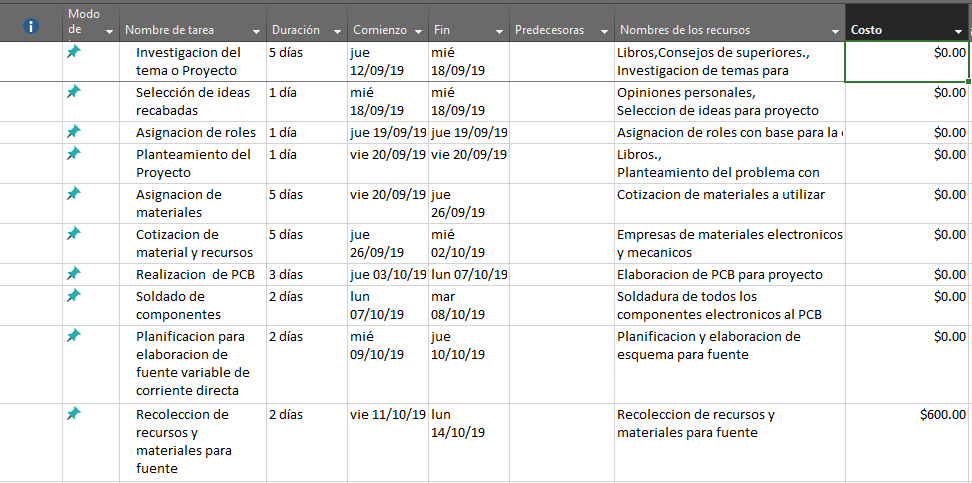
\includegraphics[width=15cm]{DefinicionTareas/4.png}\\
 
 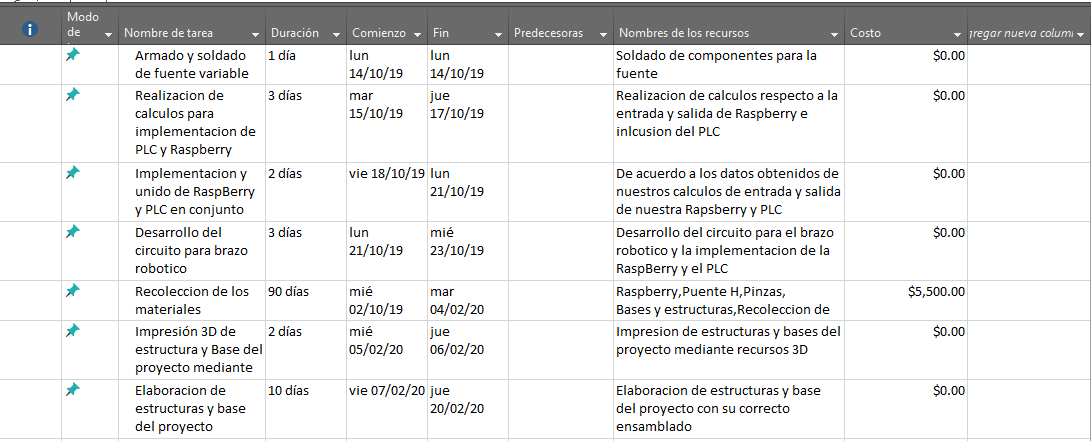
\includegraphics[width=15cm]{DefinicionTareas/5.png}\\
 
 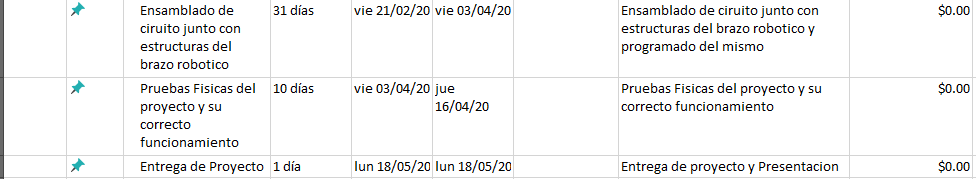
\includegraphics[width=15cm]{DefinicionTareas/6.png} 
\end{center}
\newpage
\section{Diagrama de Gantt Cronograma de Actividades y Tiempo:}
Cronograma de trabajo, fechas establecidas del 12 de  Septiembre del 2019 al dia de entrega, 18 de mayo del 2020

\begin{center}
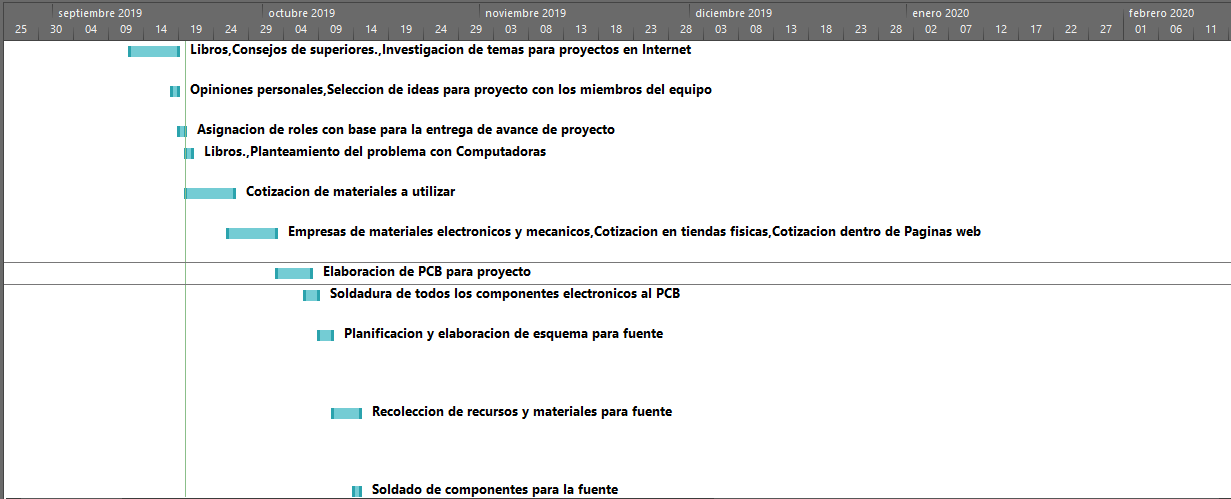
\includegraphics[width=17cm]{CronogramaTrabajo/1.png}\\

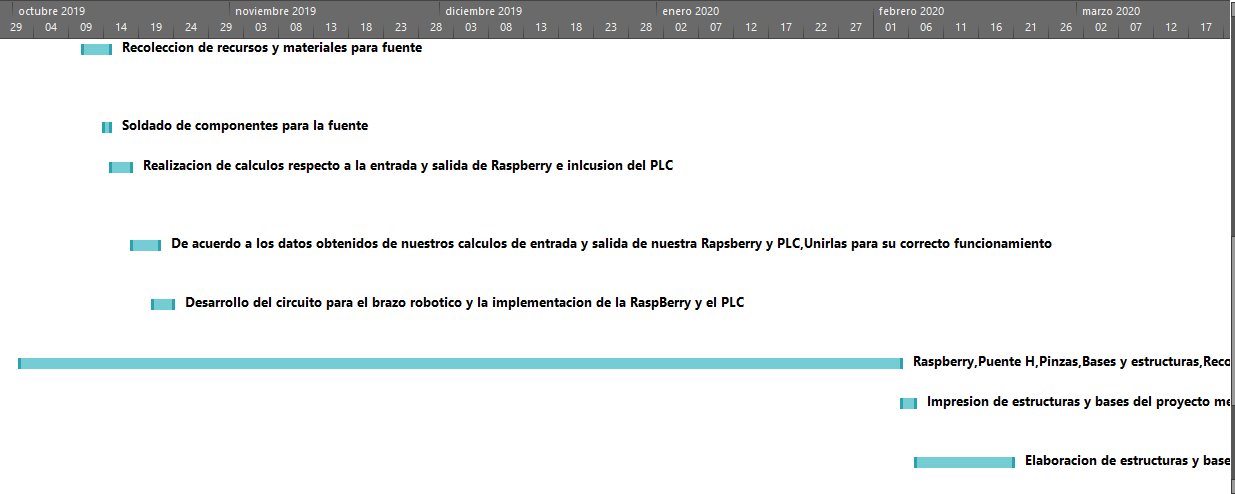
\includegraphics[width=17cm]{CronogramaTrabajo/2.png}\\

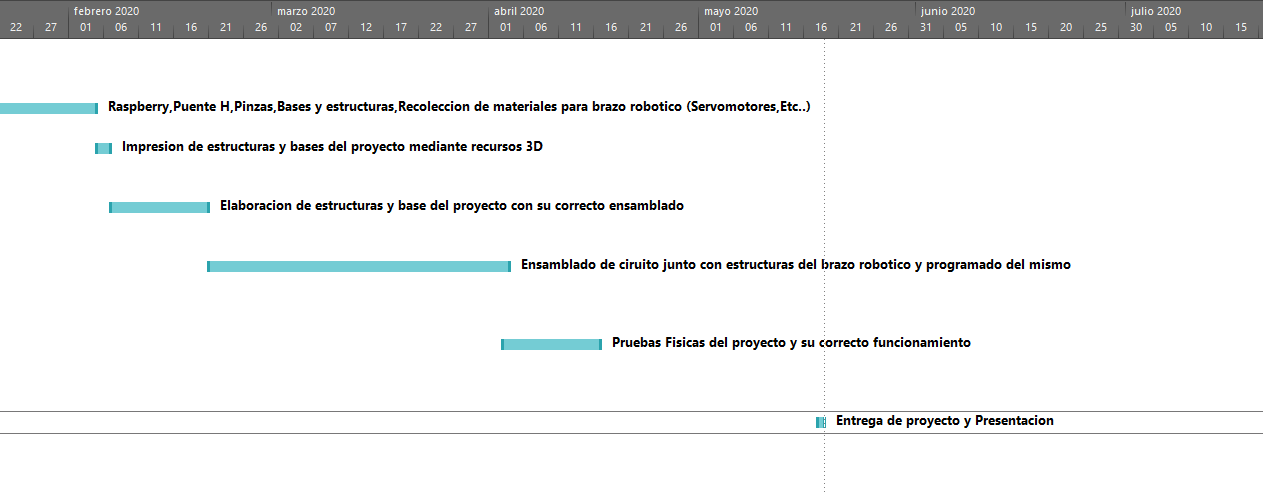
\includegraphics[width=17cm]{CronogramaTrabajo/3.png}  
\end{center}
\newpage

\section{Propuesta de Materiales:}

\subsection{Elementos consturctivos}
Manipulador o brazo mecanico.\\
Elementos motrices o actuadores.\\
Controlador.\\
Efector terminal.\\
Sensores de informacion.

\subsection{Manipulador}
Es el conjunto de elementos mecanicos que permiten el movimiento del efector termina. En la estructura interna del manipulador se encuentran ubicador muchas veces los elementos motrices, engranajes y tranmisiones que soportan el movimiento de las cuatro partes, que por lo geneal conforman el manipulador, las cuales son:\\
1-Base o pedestal de fijacion.\\
2-Cuerpo.\\
3-Brazo.\\
4-Antebrazo.\\
\subsection{Elementos motrices o Actuadores}
\paragraph{Neumaticos}
Emplean aire comprimido como fuente de energia y son adecuados en el control de movimientos rapidos, pero su precision es limitada.
\paragraph{Hidraulicos}
Los actuadores hidraulicos son recomendables en los manipuladores que tiene una gran capacidad de carga, junto a una precisa regulacion de velocidad.
\paragraph{Electricos}
Los motores electricos son los mas utilizados, gracias a su precision y la facilidad de control.
\subsection{Controlador}
Es el dispositivo encargado de regular el movimiento de todos los elementos del manipulador, y de realizar los calculos y procesado de la informacion. La complejidad del control varia segun los pramatros que se gobiernan.
\subsection{Efector Terminal}
Es la garra o herramienta que se le acopla a la muneca del manipulador, siendo el encargado de materializar el trabajo previsto por ejemplo, este puede ser una tenaza, un electroiman, o algun otro aparato. En general, y de acuerdo al tipo de aplicacion, la problematica del efector terminal radica en que este ha de posser una elevada capacidad de carga y al mismo tiempo es importante que tenga un peso y tamano reducido. Por esto, en muchas ocasiones es necesario disenar el efector terminal de acuerdo a los requerimientos de la aplicacion en que se utilizara.
\subsection{Sensores de Informacion}
Los robot inteligentes son aquellos capaces e adaptarse al ambiente y tomar decisiones en tiempo real, adecuadas para situacion. La informacion que ellos reciben les hace autoprogramables, es decir,alteran su actuar en funcion de la situacion externa, lo que los hace poseer un cierto grado de inteligencia artificial. A este respecto, las informaciones mas solicitadas por los robots son las que hacen referencia a la posicion, velocidad, aceleracion, fuerzas,pares, dimensiones y contornos de objetos, y temperatura.

\section{Presupuesto:}

\begin{tabular}{|l|l|l|l|}
\hline
	Producto & Piezas & Precio & Total\\
\hline
	Impresion 3D & 5 & 70 & 350\\

\hline
	Capacitores 33pF & 2 & 5 & 10\\
\hline
	 Circuitos integrados L293B & 2 & 15 & 30\\
\hline
	Resistencias varias & 20 & 2 & 40\\
\hline
	Diodos1N4004G & 16 & 5 & 80\\
\hline
	1 Switch & 1 & 10 & 10\\

\hline
	Fuente CA-CD & 1 & 600 & 600\\
\hline
	Push bottons & 8 & 2 & 16\\
\hline
cautin & 1 & 150 & 150\\
\hline
	Estaño & 1 & 30 & 30\\
\hline
	Multimetro & 1 & 100 & 100\\
\hline
Motores DC & 5 & 400 & 2000\\
\hline
\end{tabular}

\section{Aportacion a cada Materia:}

Ingles:\\
En este tema se estara tocando temas como la programacion que viene sustentada en ingles, asi como el reporte final de este.\\

Etica Profesional:\\
Cumpliendo las normas que se rigen en la creacion de cualquier robot, siendo sensatos de lo que estamos realizando y en que situacion lo hacemos.\\

Estructura y propiedades de los materiales:\\
Viendo la duracion y la buena prestacion que cada material que complementa el dispositivo, siendo mayor eficaz, y de utilizacion mas optima.\\

Programacion de prefifericos:\\
Implementando un programa en la web, el cual deje manejar el avance de este dispositivo, a partir de comando y compilaciones de datos almacenados en el dispositivo.\\

Sistemas electronicos de interfaz:\\
Implementando una fuente de voltaje CA-CD, el cual deje manejar en mayor eficiencia este dispositivo, complementado con diodos rectificadores, y rectificacion el cual haga manejar el voltaje que se requiere.\\

Controladores Logicos Programables:\\
En este se estara viendo todo el control que tendra el dispositivo en base, ya sea desde el movimiento y la implementacion de cada componente para que este sea de mayor sensates de rigidez, y pueda tener el manejo mas eficiente, manejado desde la terminal, y con sus componentes, en conjunto.

\section{Primer Bosquejo:}
Se ve una previsualizacion, de como quedaria establecido el proyecto a final de entrega, con algunos detallles extras que se puedan agregar en un futuro, para la mejor estetica de este.

\begin{center}
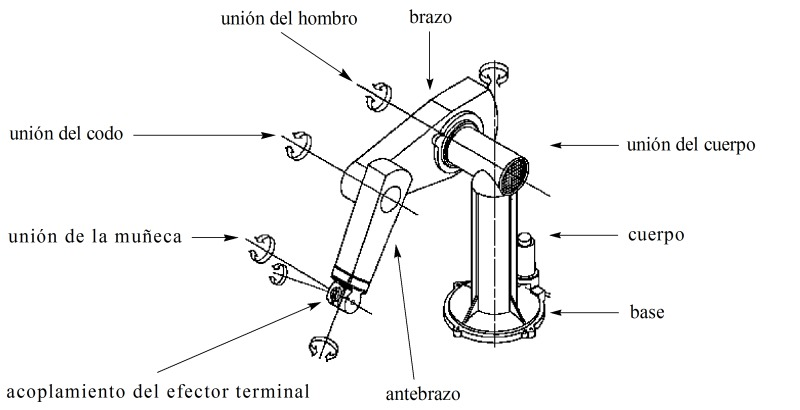
\includegraphics[width=10cm]{Bosquejo.jpeg} 
\end{center}

\section{Desarrollo:}

Lo que es el brazo robotico, puede tener muchas implementaciones a partir ya sea de una simple tarea hasta armar uanred de tareas complejas el cual, este pueda acatar sin problemas y sin ayuda de mucho trabajo, la realizacion de este proyecto se esta dando a partir de la idea de automatizacion que son los temas a tocar en este años, que se estara manejando en lo largo de este tiempo.\\
A partir de implementar todos los conocimientos recabados, en un amplio y buen funcionamiento, el cual seria el de poder dar sustento a ideas mas industriales, y de ello la innovacion de los mismos, proponiendo ideas que sean de mayor sustento y eficiencia, asi como la creacion, de un posible armado mas eficiente y barato, el cual deje a la idea de poder sustentar este tipo de proyectos, en una futura implementacion para la determinacion y elaboracion del mismo.

\section{Referencias:}
\url{www.grupoisis.uma.es/microbot/public/robots.pdf}\\

\url{http://repositorio.usfq.edu.ec/bitstream/23000/3840/1/112562.pdf}\\

\url{https://electrosite01.wordpress.com/2014/06/04/proyecto-brazo-robotico-compra-de-materiales/}\\

\url{https://www.feriadelasciencias.unam.mx/anteriores/feria21/feria361_01_desarrollo_de_brazo_robotico_para_multiples_aplica.pdf}
\end{document}